\PassOptionsToPackage{unicode,pdfusetitle}{hyperref}
\PassOptionsToPackage{hyphens}{url}
\PassOptionsToPackage{dvipsnames}{xcolor}

\documentclass[english,a4paper]{article}

\usepackage{geometry}

% Font settings
\usepackage[T1]{fontenc}
\usepackage{lmodern}
\usepackage{amssymb,amsmath,amsthm,mathtools}
\usepackage{textcomp}
\usepackage{csquotes}
\usepackage{babel}
\usepackage{upquote}

\usepackage[textsize=footnotesize]{todonotes}

\usepackage{microtype}
\UseMicrotypeSet[protrusion]{basicmath} % disable protrusion for tt fonts

% Colors
\usepackage{xcolor}

% Hyperlinks, urls, etc
\usepackage{xurl}

\usepackage{hyperref}
\hypersetup{
  colorlinks = true,
  breaklinks = true,
  linkcolor  = black,
  filecolor  = MidnightBlue,
  citecolor  = MidnightBlue,
  urlcolor   = MidnightBlue
}

\usepackage{cleveref}

% Floats
\usepackage{graphicx}
\usepackage{booktabs}
\usepackage{caption}
\usepackage{subcaption}

% Algorithms
\usepackage{algorithm,algpseudocode}

% Title Page
\usepackage[]{authblk}
\renewcommand\Affilfont{\itshape\small}

\setlength{\emergencystretch}{3em} % prevent overfull lines

% operators
\DeclareMathOperator*{\argmax}{arg\,max}
\DeclareMathOperator*{\argmin}{arg\,min}
\DeclareMathOperator{\E}{E}
\DeclareMathOperator{\var}{Var}
\DeclareMathOperator{\cov}{Cov}
\DeclareMathOperator{\tr}{tr}
\DeclareMathOperator{\diag}{diag}
\DeclareMathOperator{\range}{range}
\DeclareMathOperator{\nullspace}{null}
\DeclareMathOperator{\rank}{rank}
\DeclareMathOperator{\card}{card}
\DeclareMathOperator{\sign}{sign}
\DeclareMathOperator{\st}{S}
\DeclareMathOperator{\normal}{Normal}
\DeclareMathOperator{\fnormal}{FoldedNormal}
\DeclareMathOperator{\bernoulli}{Bernoulli}
\DeclareMathOperator{\erf}{erf}
\DeclareMathOperator{\mse}{MSE}
\DeclareMathOperator{\risk}{R}
% \DeclareMathOperator{\I}{I}
% \DeclareMathOperator{\T}{}
%
% \DeclareMathSymbol{\phi}{\mathalpha}{operators}{0}
\DeclareMathOperator{\pdf}{\phi}
\DeclareMathOperator{\cdf}{\Phi}
% commands
% \newcommand{\vec}{\vectorsym}
% \newcommand{\mat}{\matrixsym}
\renewcommand{\vec}{\boldsymbol}
\newcommand{\mat}{\boldsymbol}
\newcommand*\du{\mathop{}\!\mathrm{d}}
% \newcommand{\T}{\mathsf{T}}
\newcommand{\T}{\intercal}
\newcommand{\ones}{\boldsymbol{1}}
% \newcommand{\T}{\intercal}
% \newcommand{\T}[1]{{1}^{\mathsf{T}}}
\newcommand{\ind}[1]{\operatorname{I}_{#1}}

% environments
\theoremstyle{plain}
\newtheorem{theorem}{Theorem}[section]
\newtheorem{corollary}{Corollary}[theorem]
\newtheorem{lemma}{Lemma}[section]
\newtheorem{proposition}{Proposition}[section]

\theoremstyle{definition}
\newtheorem{definition}{Definition}[section]
\newtheorem{example}{Example}[section]

\theoremstyle{remark}
\newtheorem{remark}[theorem]{Remark}

\newcommand{\todojl}[1]{\todo[color=green!40]{#1}}



% title block
\title{Standardization and Regularization}
\author[1,*]{Johan Larsson}
\affil[1]{Department of Statistics, Lund University}
\affil[*]{Corresponding author:
  \href{mailto:johan.larsson@stat.lu.se}{\nolinkurl{johan.larsson@stat.lu.se}}
}
\date{\today}

% % bibliography
% \makeatletter
% \def\blx@nowarnpolyglossia{}
% \makeatother
% \usepackage[citestyle=alphabetic,language=english]{biblatex}
% \addbibresource{normreg.bib}

\begin{document}

\maketitle

\section{Introduction}

When the data you want to model is high-dimensional, that is, the number of features \(p\) exceed the number of observations \(n\), it is impossible to apply classical statistical models such as standard linear regression since the design matrix \(\mat X\) is no longer of full rank. A common remedy to this problem is to \emph{regularize} the model by adding a term to the objective function that punishes models with large coefficients (\(\vec\beta\)). If we let \(h(\vec\beta; \mat X, \vec y)\) be the original objective function---which when minimized improves the model's fit to the data (\(\mat X, \vec y\))---then
\[
  f(\beta_0, \vec\beta; \mat X, \vec y) = h(\beta_0, \vec\beta; \mat X, \vec y) + g(\vec\beta)
\]
is a composite function within which we have added a penalty term \(g(\vec\beta)\). As you can see, this penalty term, in contrast to \(h\), depends only on the coefficients (in fact typically only on the absolute values thereof).

Some of the most common penalties are the \(\ell_1\) and \(\ell_2\) penalties, that is \(g(\vec\beta) = \lVert \vec\beta \rVert_1\) or \(g(\vec\beta) = \lVert \vec\beta \rVert_2^2/2\)\footnote{Division by two in this case is used only for convenience.}, which, if \(h\) is the standard ordinary least-squares objective, result in lasso and ridge (Tikhonov) regression respectively. Other common penalities include SLOPE, MCP, and SCAD. Many of these penalities---in fact all of the previously mentioned ones---penalize coefficients through shrinkage.

% TODO: Maybe say something about ℓ₀ (best subset) regularization?

The problem with this type of regularizing is that the penalty term \(g\) is sensitive to the scales of the features in \(\mat X\). As a initial example of this, let us take \(h\) to be the lasso objective, where \(f\) is the ordinary least-squares objective and \(h\) the \(\ell_1\) norm and consider a one-dimensional problem, that is, the composite objective is
\[
  \frac{1}{2} \sum_{i=1}^n(y_i - \beta_0 - \vec{x}^T_i \vec\beta)^2 + \lambda \lvert \vec\beta \rvert.
\]

Next, we introduce a scaling matrix \(\mat S = \diag(s_1, s_2, \dots, s_p)\), with \(s_j > 0\) and an \(n \times p\) large translation matrix \(\mat T\) where \(t_{ij} = t_{kj}\) for all \(i,k \in [n]\). Then \(\tilde{\mat X} = (\mat X - \mat T) \mat S^{-1}\) is the normalized design matrix.

\begin{example}
  If \(s_j\) and \(t_j\) are the standard deviation and sample mean of the \(j\)th column of \(\mat X\) respectively, then \(\tilde{\mat X}\) is the standardized design matrix.
\end{example}

\begin{proposition}
  If \(\mat X^\T \mat X\) is diagonal, then
  \[
    \hat{\beta}_j = \frac{s_j\softthreshold\big((\vec x_j - \vec{1}t_j)^\T\vec{y}; s_j\lambda\big)}{\lVert \vec x_j - \vec{1}t_j\rVert_2^2} \text{ for all } j \in [p],
  \]
  where \(\softthreshold(\beta; \lambda) = \sign(\beta)\max\big(\lvert \beta \rvert - \lambda, 0\big)\) is the \emph{soft thresholding operator}.
\end{proposition}
\begin{proof}
  The KKT stationarity condition for the normalized lasso problem is
  \[
    \vec{0} \in \tilde{\mat{X}}^\T(\tilde{\mat{X}}\vec{\beta} - \vec{y}) + \lambda g,
  \]
  where \(g\) is the subgradient of the \(\ell_1\) norm.
  If \(\mat{X}^\T\mat{X}\) is diagonal, then this condition resolves into \(p\) piecewise conditions given by
  \[
    0 \in \tilde{\vec{x}}_j^\T\tilde{\vec{x}}_j\beta_j - \tilde{\vec{x}}_j^\T\vec{y} + \lambda g \quad \forall\, j \in [p]\).
  \]
  The subdifferential of the \(\ell_1\) norm is \([-1, 1]\), that is, \(g \in [-1, 1]\), and it is well-known that the solution to the equation above is
  given by
  \[
    \frac{\softthreshold(\tilde{\vec{x}}_j^\T \vec{y}; \lambda)}{\lVert \tilde{\vec{x}}_j\rVert_2^2} =
    \frac{s_j\softthreshold\big((\vec{x}_j - \vec{1}t_j)^\T\vec{y}; s_j\lambda\big)}{\lVert \vec{x}_j - \vec{1}t_j\rVert_2^2}.
  \]
\end{proof}

\section{Binary Data}

Normalization attempts to place variables on a similar---optimally identical---scale. In the case when all the features come from continuous variables and particularly if they are, for instance, normally distributed, succeeding in this is reasonable to assume. But it is harder to justify in the case when the features are composed of a mix of binary and continuous data.

For simplicity, let's start by assuming that we have a two-dimensional problem and that \(x_{i1} \sim \bernoulli(p)\) and \(x_{i2} \sim \normal(0, 1)\) with no dependence. When \(p = 0.5\), that is, classes are completely balanced, then the population standard deviation for \(\vec{x}_2\) is 0.5 and for \(x_1\) 1. After standardization, values for \(\vec{x}_2\) will lie between 0 and 2, with a standard deviation of 1. For \(\vec{x}_2\), 69\% of the values will lie between an equally spaced range, -1 to 1, and the standard deviation will of course also be 1. We will not discuss whether this is a reasonable way to normalize these two variables; there is certainly justification for it, but it's not obvious that it is the best way for all data.

A definite issue arises, however, as

\begin{figure}[htpb]
  \centering
  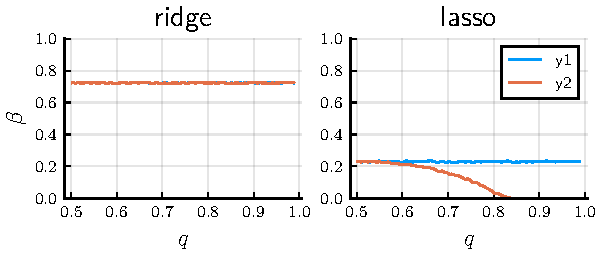
\includegraphics[]{plots/dummy-plot.pdf}
  \caption{%
    Comparison between lasso and ridge estimators for a two-dimensional problem where one feature is generated from \(\bernoulli(q)\) and the other from \(\normal(0, 0.5)\). The ridge estimator is unaffected by \(q\), but the lasso estimator is not.
  }
  \label{fig:}
\end{figure}

\section{To Do}

\begin{itemize}
  \item Use homotopy path algorithm to express upcoming critical \(\lambda\) values as a function oDiscussing whether or not this is a reasonable transformation that indeed should place these variables on a similar scale is f the scaling of the features.
  \item Solve two-dimensional ridge regression problem with correlation to examine the effects of correlation between a binary and a continuous variable.
  \item Solve a two-dimensional lasso problem, without correlation, to observe the relative effect of standard deviation.
  \item Use Fisher–Tippett–Gnedenko theorem to say something about the effect of max-abs-scaling when used with gaussian and bernoulli variables.
  \item Consider the relationship to adaptive lasso.
\end{itemize}

\section{Insights}

\begin{itemize}
  \item Rare traits (especially in binary data), will ``never'' be selected
  \item Outliers can cause variables to not be selected.
  \item Scaling with maximum absolute value means that for a Gaussian variable, the importance of a variable decrease with the number of samples (since the change of encountering a high value increases).
\end{itemize}

\section{Open Questions}

\begin{itemize}
  \item What effect does standardization have when it is used in the presence of dummy variables?
  \item Should dummy variables be standardized?
  \item In which situations is standardization of type x useful? What about type y?
  \item Is this only a problem for simpler models? I.e., does it matter for neural networks, for instance? Probably not.
  \item What about optimization?
  \item Adaptive lasso can be seen as a type of pre-processing. How does it compare? Does it fix the problems here?
  \item We standardize unconditionally, but interpret regression coefficients conditionally
  \item Can we quantify how strong a given feature's RMSE needs to be for it to be selected?
  \item How is prediction performance affected by this?
  \item How is false discovery rate affected by this?
  \item How is cross-validation affected by this?
  \item Can we mitigate the effect through stratification of the features?
  \item Can we mitigate the effect through some type of normalization?
\end{itemize}

% \printbibliography

\end{document}
